% Options for packages loaded elsewhere
\PassOptionsToPackage{unicode}{hyperref}
\PassOptionsToPackage{hyphens}{url}
%
\documentclass[
]{article}
\usepackage{lmodern}
\usepackage{amssymb,amsmath}
\usepackage{ifxetex,ifluatex}
\usepackage{graphicx}
\ifnum 0\ifxetex 1\fi\ifluatex 1\fi=0 % if pdftex
  \usepackage[T1]{fontenc}
  \usepackage[utf8]{inputenc}
  \usepackage{textcomp} % provide euro and other symbols
\else % if luatex or xetex
  \usepackage{unicode-math}
  \defaultfontfeatures{Scale=MatchLowercase}
  \defaultfontfeatures[\rmfamily]{Ligatures=TeX,Scale=1}
\fi
% Use upquote if available, for straight quotes in verbatim environments
\IfFileExists{upquote.sty}{\usepackage{upquote}}{}
\IfFileExists{microtype.sty}{% use microtype if available
  \usepackage[]{microtype}
  \UseMicrotypeSet[protrusion]{basicmath} % disable protrusion for tt fonts
}{}
\makeatletter
\@ifundefined{KOMAClassName}{% if non-KOMA class
  \IfFileExists{parskip.sty}{%
    \usepackage{parskip}
  }{% else
    \setlength{\parindent}{0pt}
    \setlength{\parskip}{6pt plus 2pt minus 1pt}}
}{% if KOMA class
  \KOMAoptions{parskip=half}}
\makeatother
\usepackage{xcolor}
\IfFileExists{xurl.sty}{\usepackage{xurl}}{} % add URL line breaks if available
\IfFileExists{bookmark.sty}{\usepackage{bookmark}}{\usepackage{hyperref}}
\hypersetup{
  pdftitle={CSCM37: Coursework 1},
  pdfauthor={Andrew Gray (445348)},
  hidelinks,
  pdfcreator={LaTeX via pandoc}}
\urlstyle{same} % disable monospaced font for URLs
\setlength{\emergencystretch}{3em} % prevent overfull lines
\providecommand{\tightlist}{%
  \setlength{\itemsep}{0pt}\setlength{\parskip}{0pt}}
\setcounter{secnumdepth}{-\maxdimen} % remove section numbering

\title{CSCM37: Coursework 1}
\author{Andrew Gray \\(445348)}
\date{25/02/2020}

\begin{document}
\maketitle

\hypertarget{part-1-design-1}{%
\section{Part 1, design 1}\label{part-1-design-1}}

\begin{figure}
\centering

\caption{Design 1}
\end{figure}

\hypertarget{description}{%
\subsubsection{Description}\label{description}}

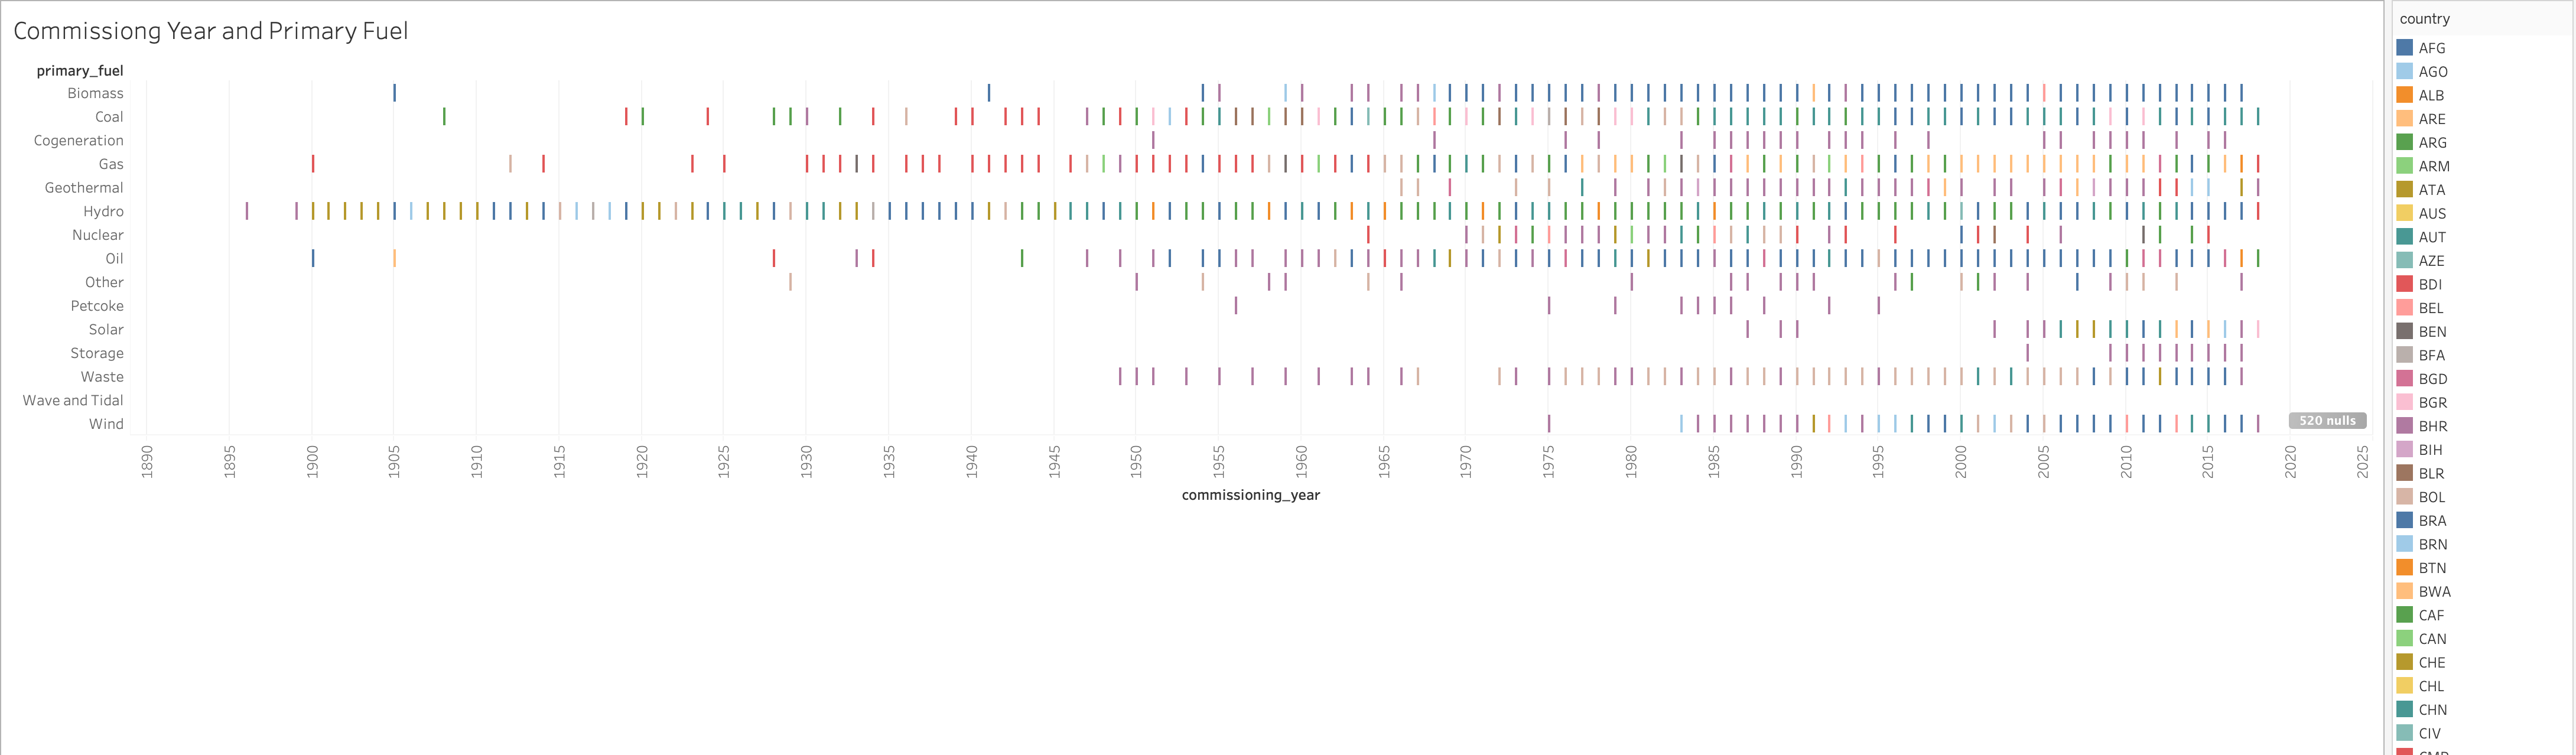
\includegraphics[width=15cm]{Viz1.png}

\begin{description}
\item[Visual Design Type:]
Gantt
\item[Name of Tool:]
Tableua
\item[Country:]
All Countries
\item[Year:]
1896 - 2018
\item[Visual Mappings:]
\begin{itemize}
\tightlist
\item
  \textbf{mapping 1}: ???
\end{itemize}

\begin{itemize}
\tightlist
\item
  \textbf{mapping 2}: ???
\end{itemize}
\item[Unique Observation:]
The oldest powerplant was commissioned in the USA in 1896 and its main fuel type was hydo. The second commissioned powerplant was also in the USA and again this was hydo which was commissioned in the 1899. Then in 1900 3 power plants were commissioned. These were Brazil - , -, -.

\item[Data Preparation:]
There was no modifications made to this dataset.
\end{description}

\hypertarget{part-1-design-2}{%
\section{Part 1, design 2}\label{part-1-design-2}}

\centering
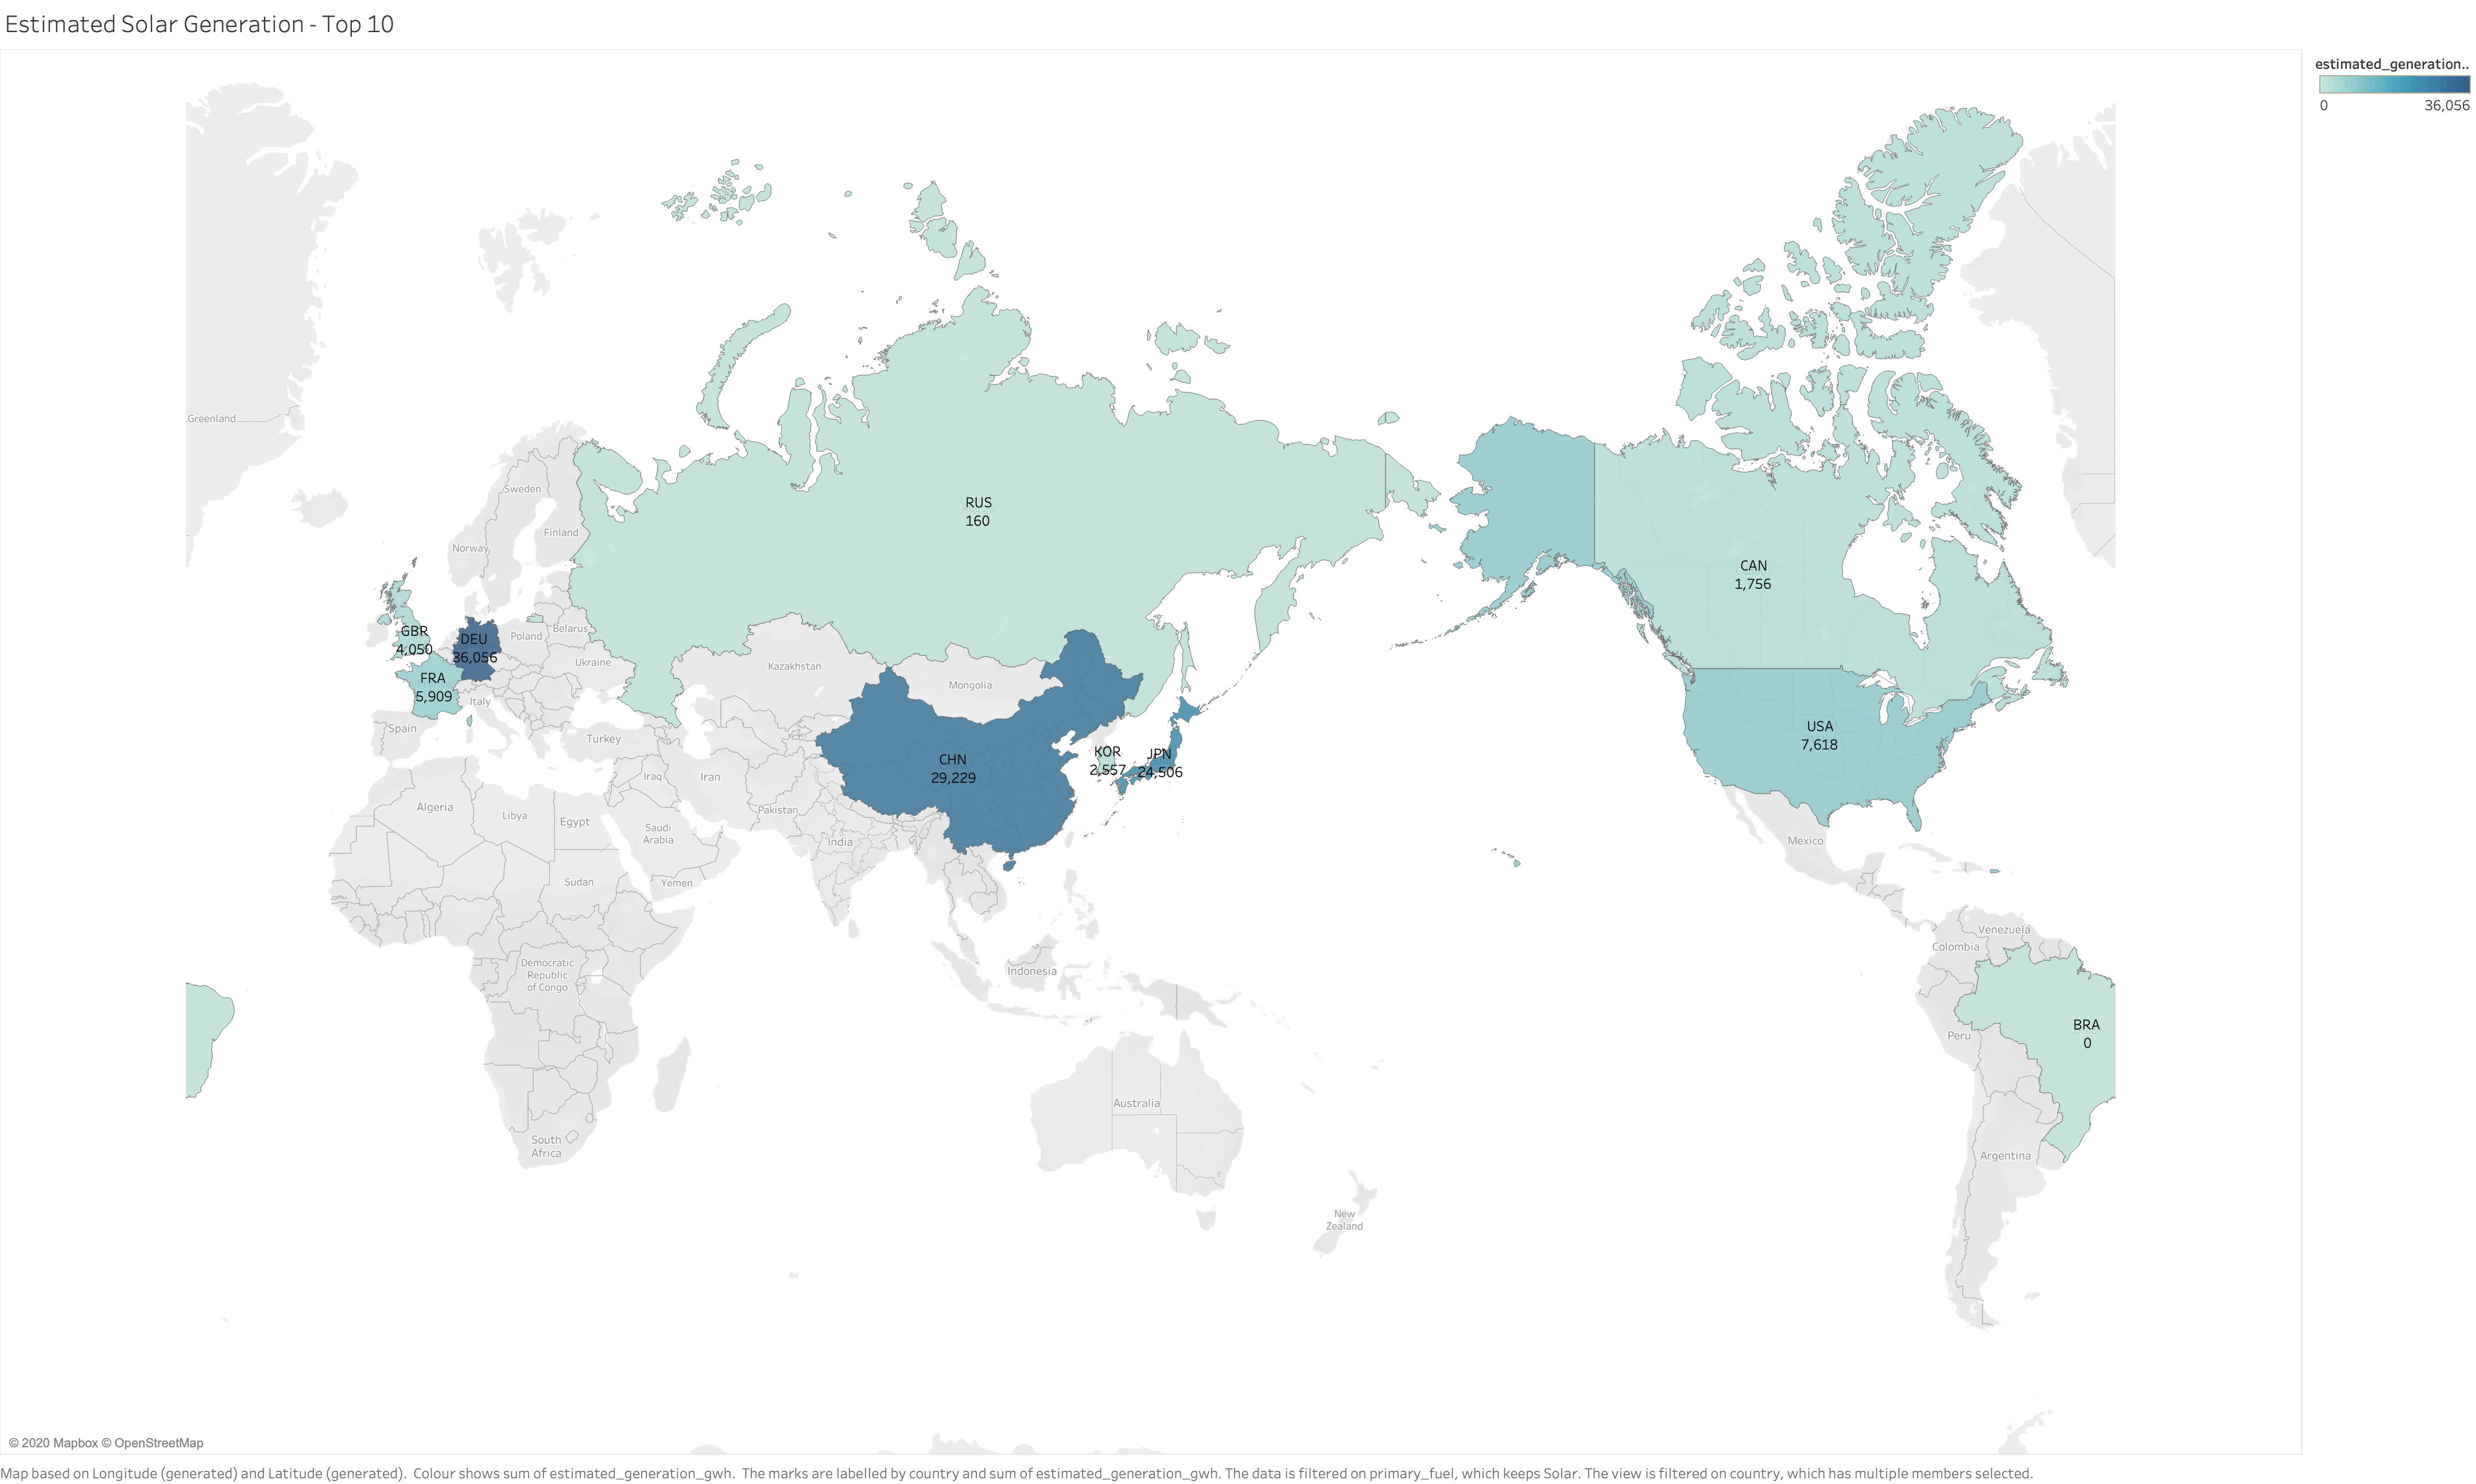
\includegraphics[width=15cm]{Viz2.png}

\hypertarget{description}{%
\subsubsection{Description}\label{description}}

\begin{description}
\item[Visual Design Type:]
Map
\item[Name of Tool:]
Tableua
\item[Country:]
France, Germany, Great Britain, Russia, China, Japan, South Korea, USA, Canada, Brazil.
\item[Year:]
2018
\item[Visual Mappings:]
\begin{itemize}
	\tightlist
	\item[  ]
\end{itemize}
\begin{itemize}
\tightlist
\item
  \textbf{mapping 1}: X and Y axis use the longitude and latitude values, this produces the map.
\end{itemize}

\begin{itemize}
\tightlist
\item
  \textbf{mapping 2}: Country is used to label the visualisation as well as the text. Colour is used to give a scale of the values, with dark being the biggest and a lighter colour being the smallest.
\end{itemize}
\item[Unique Observation:]
Germany is estimated to have the highest amount of solar energy created in 2018, at a value of 36,056. China is the second biggest estimation of solar power generated.

Weirdly enough, most counties around the equator are not in the top 10 of solar power energy generated. Brazil being the only one. You would think that this would be an effective source to tap into.

\item[Data Preparation:] Two filters have been applied, primary fuel, which is set to solar and country, which just shows the top 10 based on the sum of the estimated generation of energy.
\end{description}  
\hypertarget{part-1-design-3}{%
\section{Part 1, design 3}\label{part-1-design-3}}

\centering
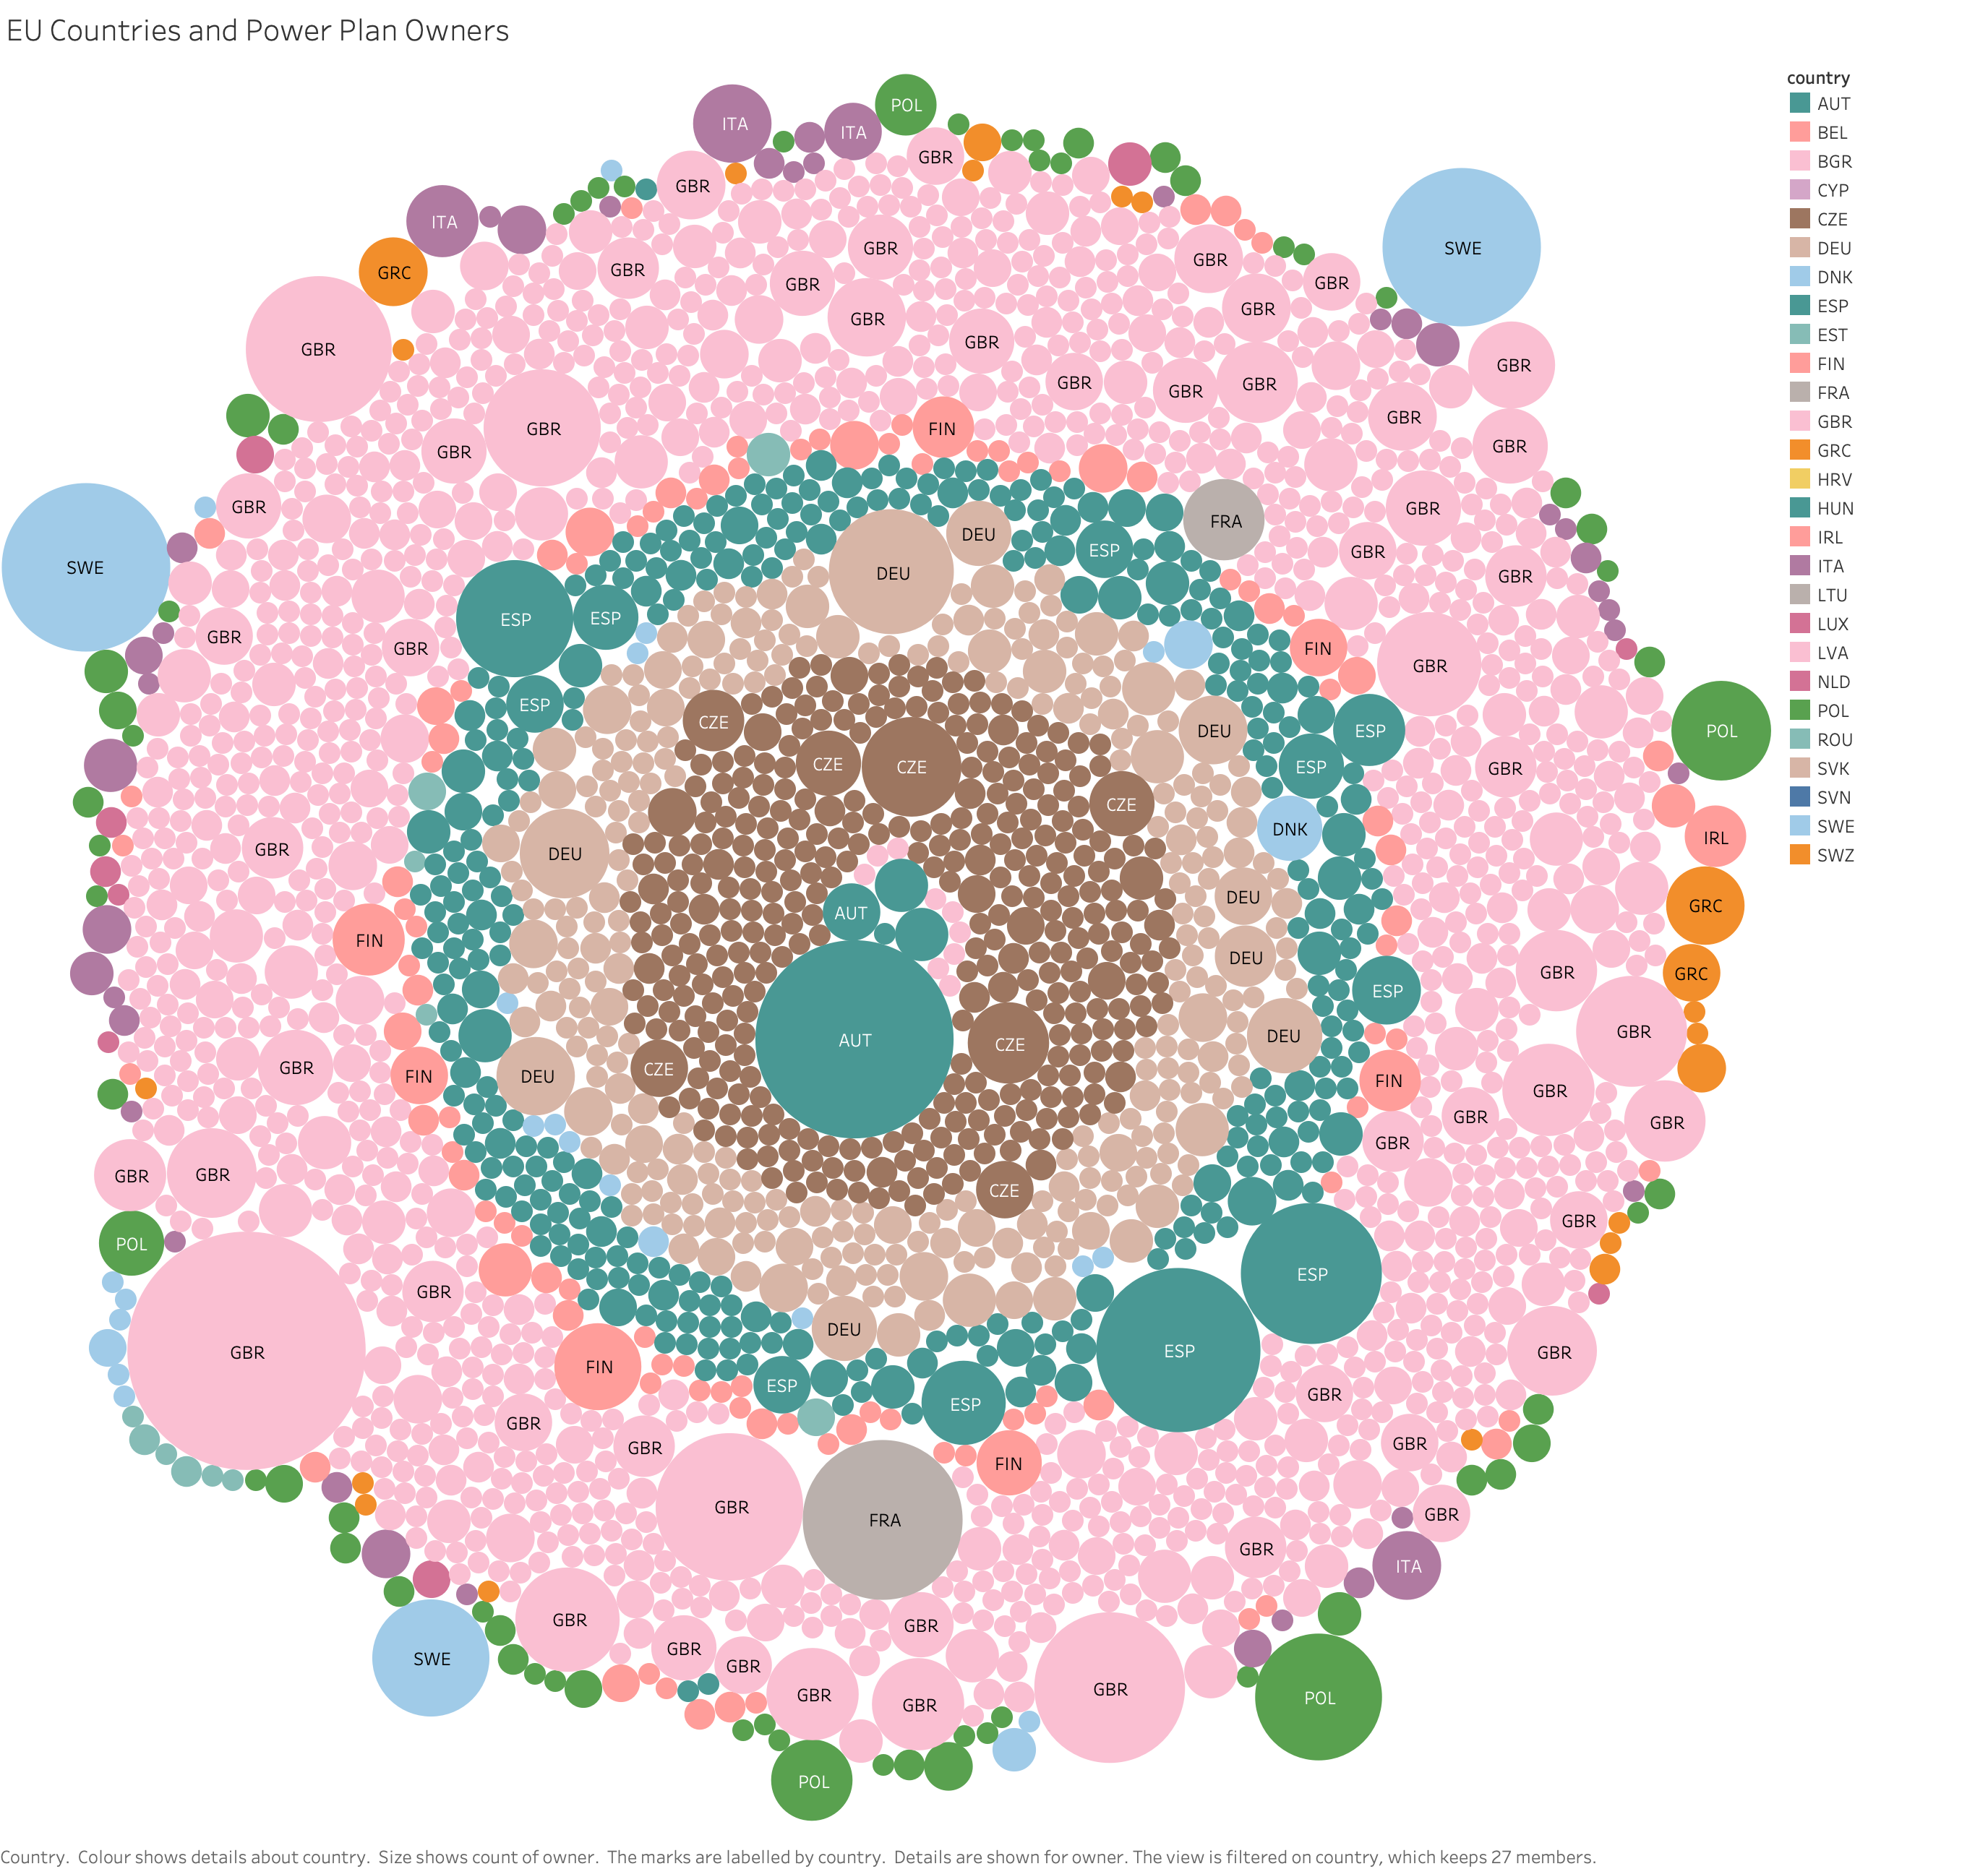
\includegraphics[height=10cm]{Viz3.png}

\hypertarget{description}{%
\subsubsection{Description}\label{description}}

\begin{description}
\item[Visual Design Type:]
Packed Bubbles
\item[Name of Tool:]
Tableau
\item[Country:]
EU members including the UK.  Austria, Belgium, Bulgaria, Cyprus, Czech Republic, Germany, Denmark, Estonia, Spain, Finland, France, United Kingdom, Greece, Croatia, Hungary, Ireland, Italy, Lithuania, Luxembourg, Latvia, Malta, Netherlands, Poland, Portugal, Romania, Sweden, Slovenia, Slovakia.
\item[Year:]
1896 - 2018
\item[Visual Mappings:]
\begin{itemize}
	\tightlist
	\item[  ]
\end{itemize}
\begin{itemize}
\tightlist
\item
  \textbf{mapping 1}: The count of the owner was used to generate the size of the bubbles. 
\end{itemize}

\begin{itemize}
\tightlist
\item
  \textbf{mapping 2}: The owner was also used as a detail as well as the sum of the number of records on the visualisation. Country was used for the colour coding and also used for the tooltip.
\end{itemize}
\item[Unique Observation:]
All of France’s power plants are owned by two companies, EDF and GDF-Suez. While the Great Britton has the most amount of different owners for their power plants.
\item[Data Preparation:]
Data was filtered by country.
\end{description}
\hypertarget{part-1-design-4}{%
\section{Part 1, design 4}\label{part-1-design-4}}

\centering
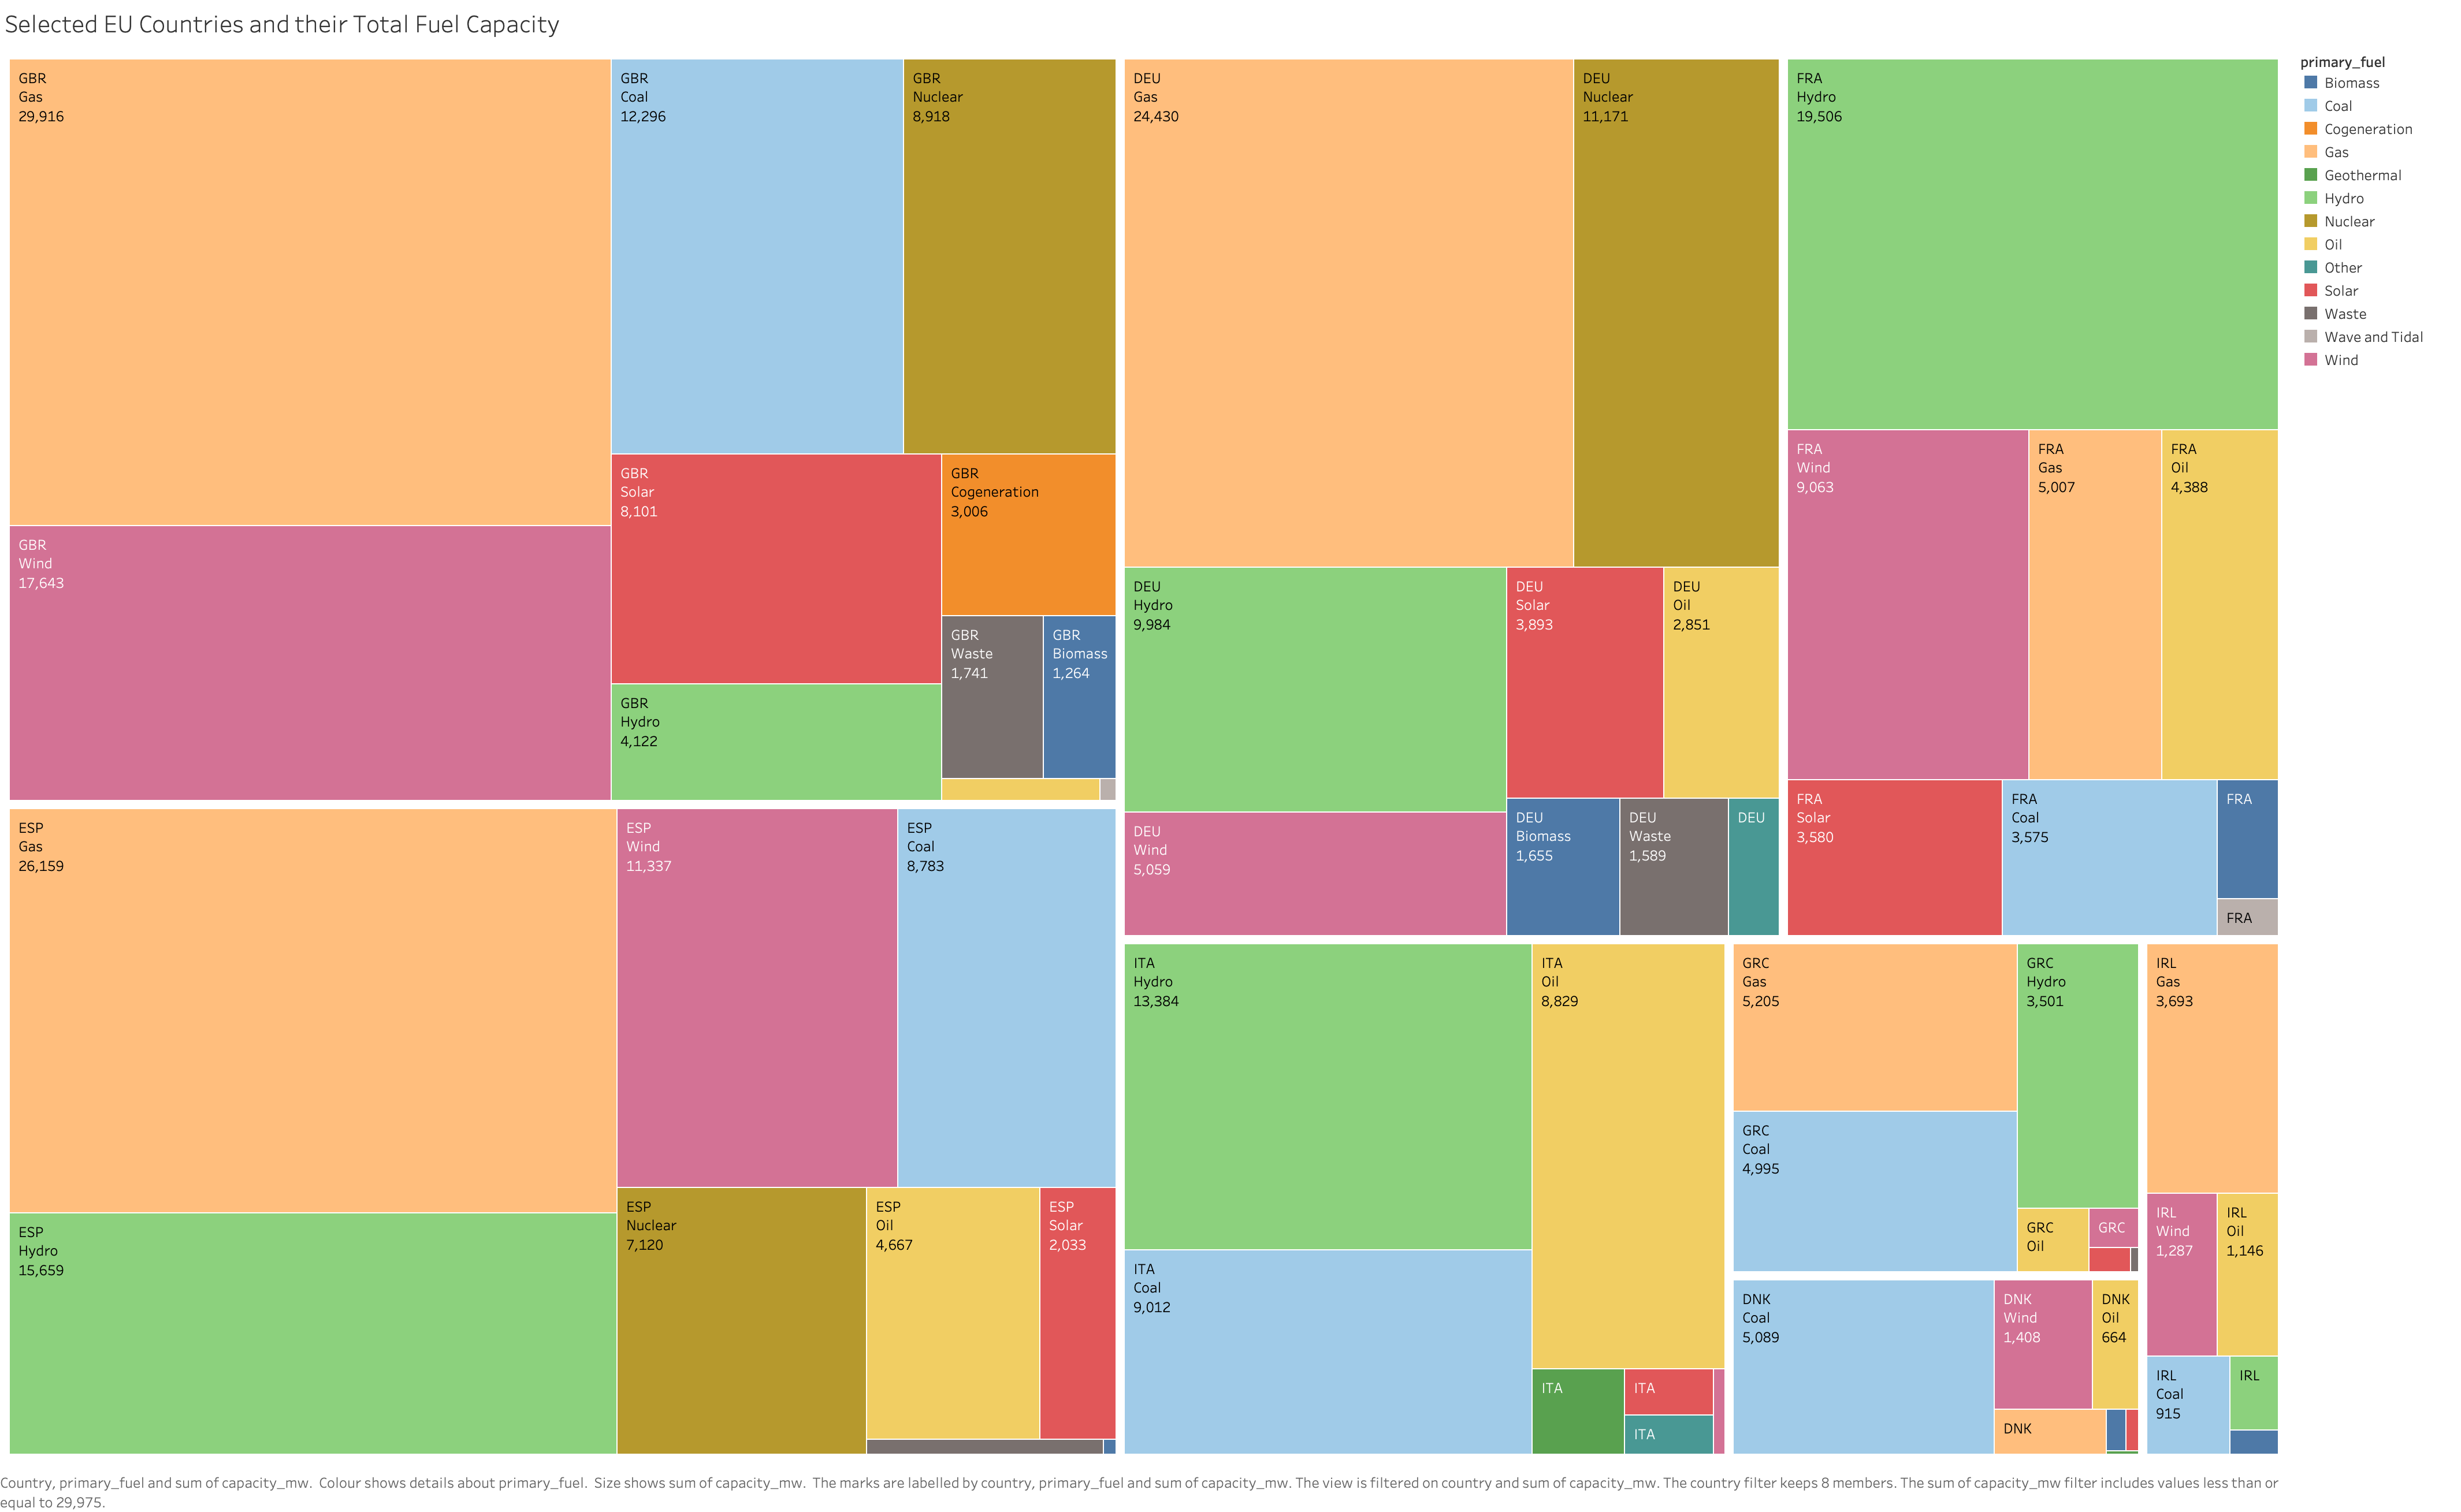
\includegraphics[width=15cm]{Viz4.png}

\hypertarget{description}{%
\subsubsection{Description}\label{description}}

\begin{description}
\item[Visual Design Type:]
Treemap
\item[Name of Tool:]
Tableau
\item[Country:]
Great Brittan, Spain, Germany, Italy, France, Greece, Denmark, Ireland.
\item[Year:]
2018
\item[Visual Mappings:]
\begin{itemize}
	\tightlist
	\item[  ]
\end{itemize}

\begin{itemize}
\tightlist
\item
  \textbf{mapping 1}: Primary fuel was used for the colour coding.
\end{itemize}
\begin{itemize}
	\tightlist
	\item
	\textbf{mapping 2}: sum of the capacity was used for the size.
\end{itemize}
\begin{itemize}
\tightlist

\item
  \textbf{mapping 3}: Country, primary fuel and sum of the capacity was used as a label within the visualisation.
\end{itemize}
\item[Unique Observation:]
France has the most amount of energy capacity. The largest of the capacity being for nuclear energy with a capacity of 63,130. The country with the next amount of capacity is Germany with Coal being its primary fuel at 47,773.
\item[Data Preparation:]
A filter on the countries listed has been used.
\end{description}
 

\hypertarget{part-1-design-5}{%
\section{Part 1, design 5}\label{part-1-design-5}}

\centering
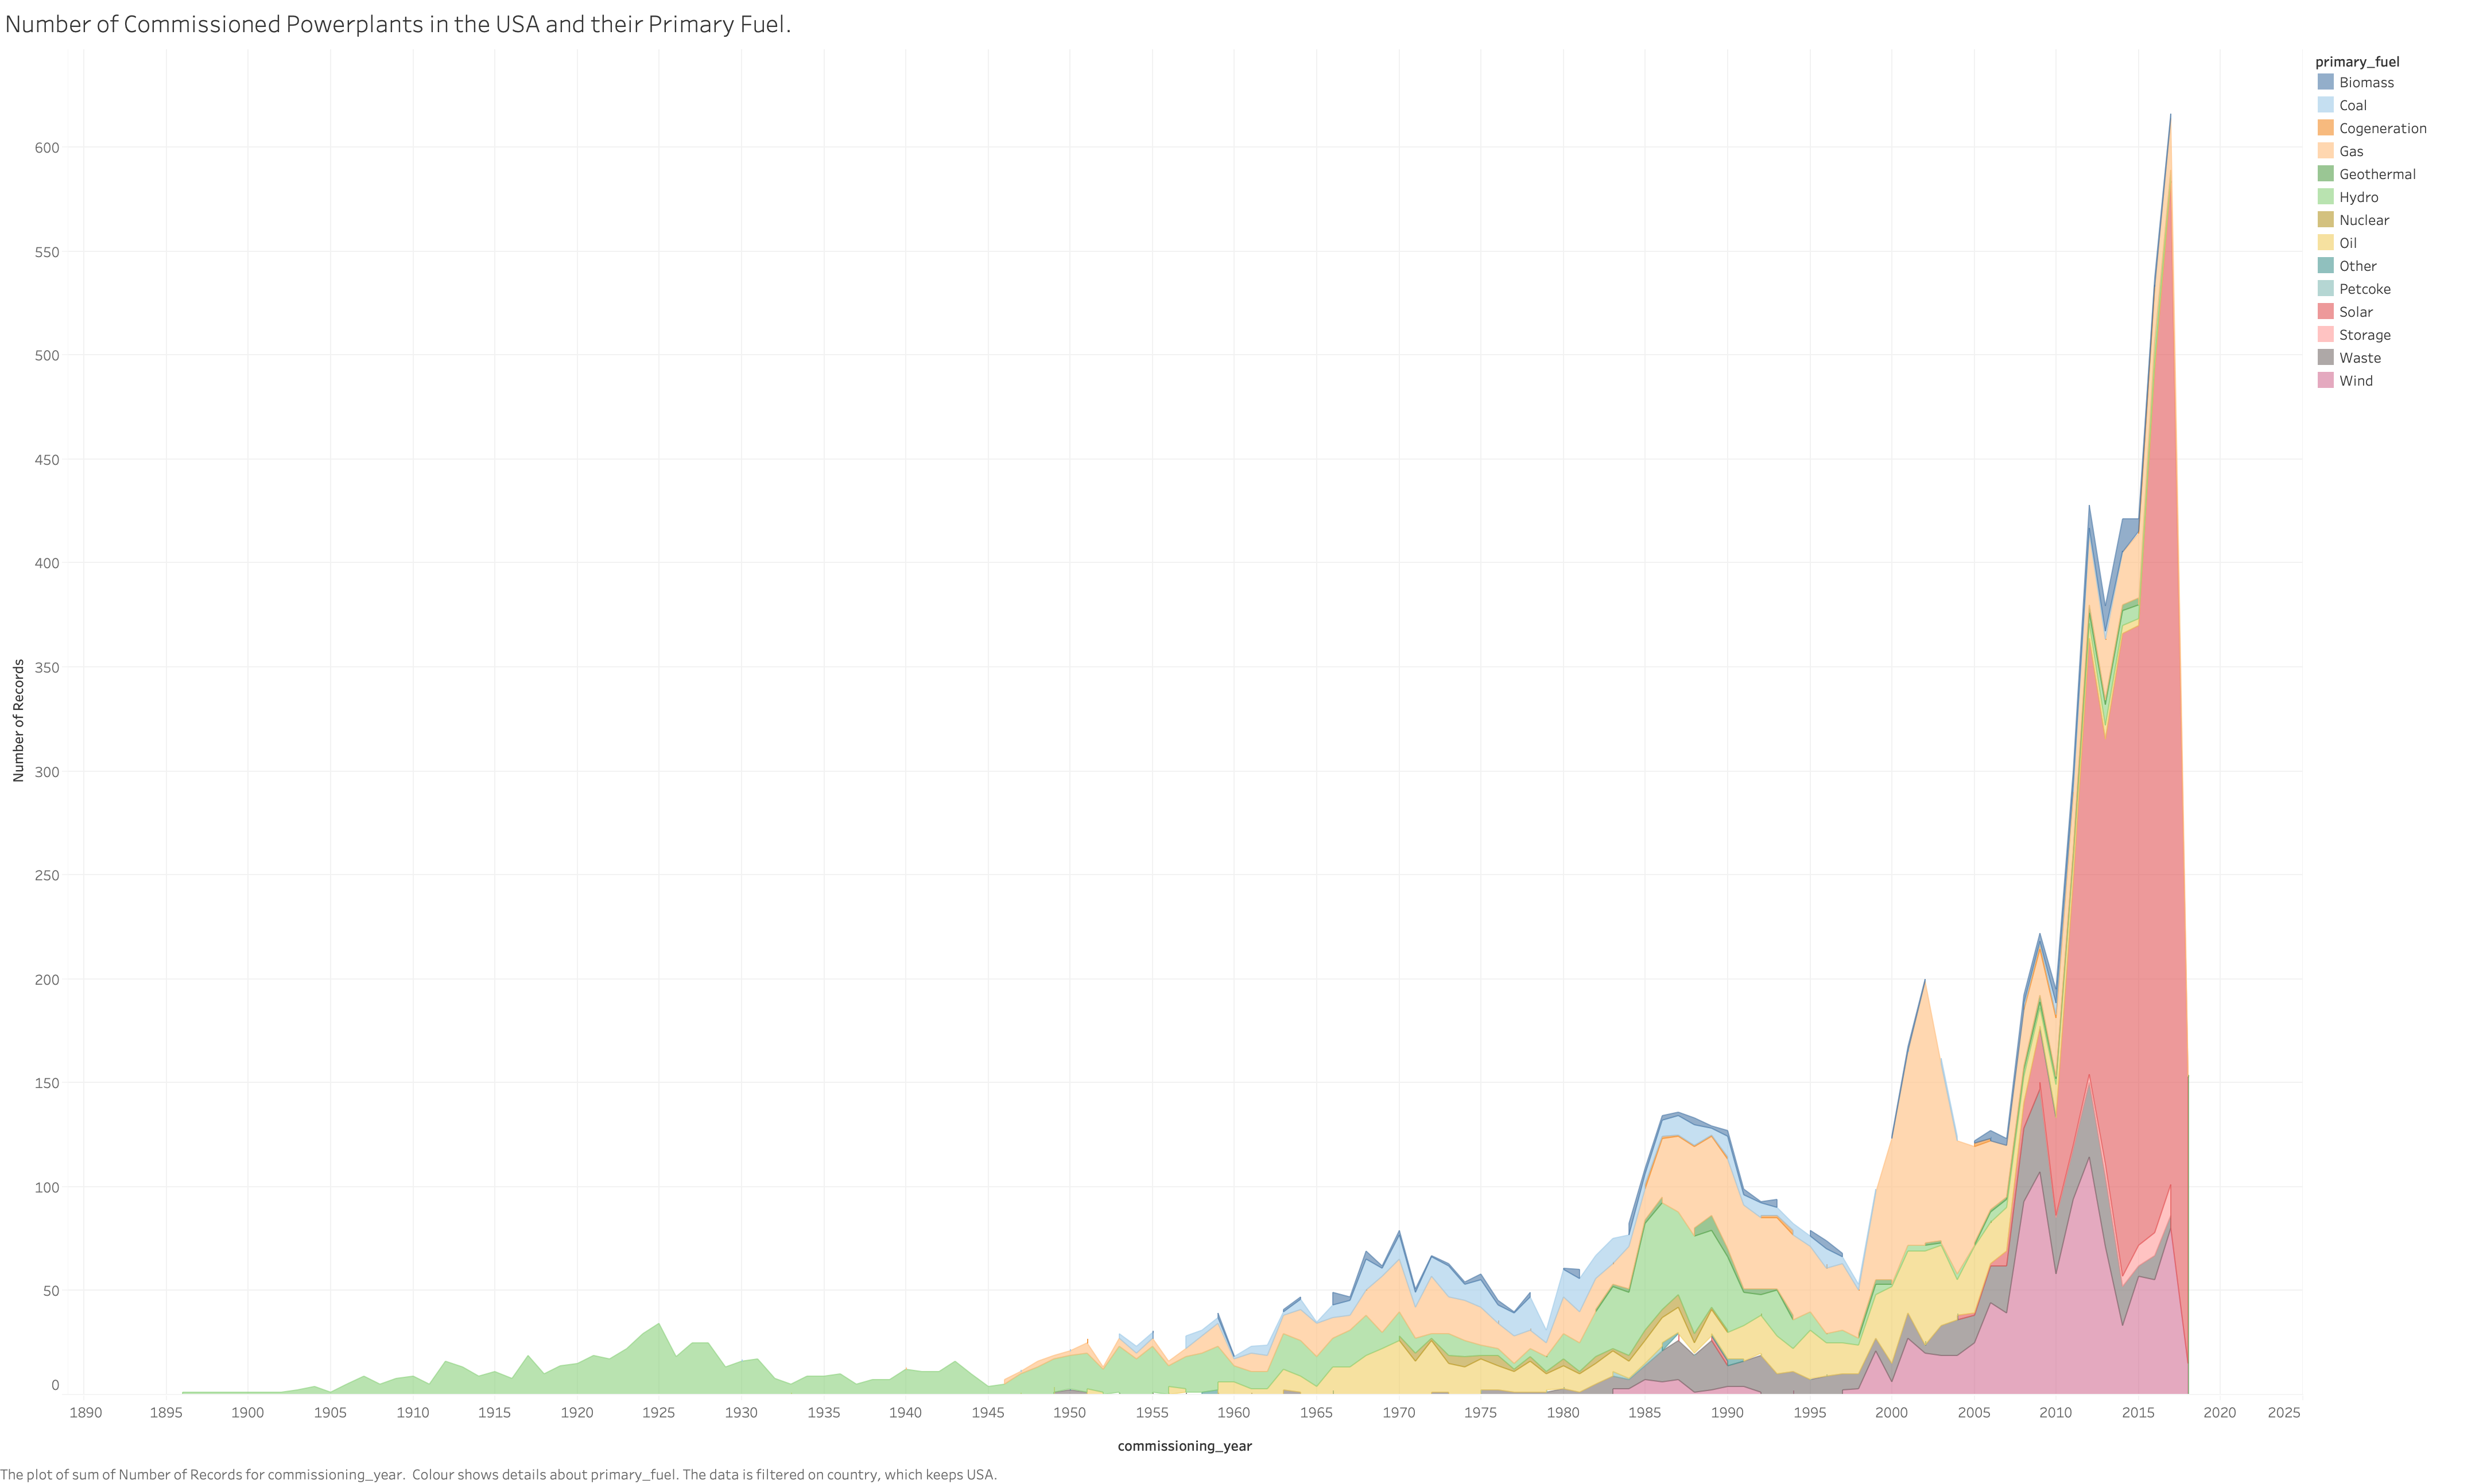
\includegraphics[width=15cm]{Viz5.png}

\hypertarget{description}{%
\subsubsection{Description}\label{description}}

\begin{description}
\item[Visual Design Type:]
Area Charts Continuous.
\item[Name of Tool:]
Tableau
\item[Country:]
USA
\item[Year:]
1890 - 2018
\item[Visual Mappings:]
\begin{itemize}
	\tightlist
	\item[  ]
\end{itemize}
\begin{itemize}
\tightlist
\item
  \textbf{mapping 1}: X is assigned to commissioning year and the y axis is assigned to the sum of the number of records.
\end{itemize}

\begin{itemize}
\tightlist
\item
  \textbf{mapping 2}: The colour of the area charts are assigned to the primary fuels.
\end{itemize}
\item[Unique Observation:]
Between 1896 - 1946 the USA only every commissioned hydro power plants.
\item[Data Preparation:]
Data filtered to only show USA.
\end{description} 

\clearpage
\hypertarget{part-2-treemap-1}{%
\section{Part 2, Treemap 1}\label{part-2-treemap-1}}

\begin{figure}
\centering
%\includegraphics{imagepath}
\caption{Treemap 1}
\end{figure}

\begin{itemize}
\tightlist
\item
  \textbf{Name of Tool}: The tool that was used to generate the treemap
\item
  \textbf{Country}: Name of country(s) data shown
\item
  \textbf{Year}: the year(s) or time-span of data shown
\item
  \textbf{Data Preparation}: A helpful description of how you prepared
  the data
\item
  \textbf{Color}: what is color mapped to?
\item
  \textbf{Hierarchy}: What is the data hierarchy contained in the
  treemap?
\item
  What leaf node size is mapped to?
\item
  How are the leaf nodes laid out or positioned?
\item
  What are internal nodes mapped to?
\item
  What is internal node size mapped to?
\item
  Which treemap node layout algorithm is used?
\end{itemize}

%\hypertarget{part-2-treemap-2}{%
\section{Part 2, Treemap 2}\label{part-2-treemap-2}}

\centering
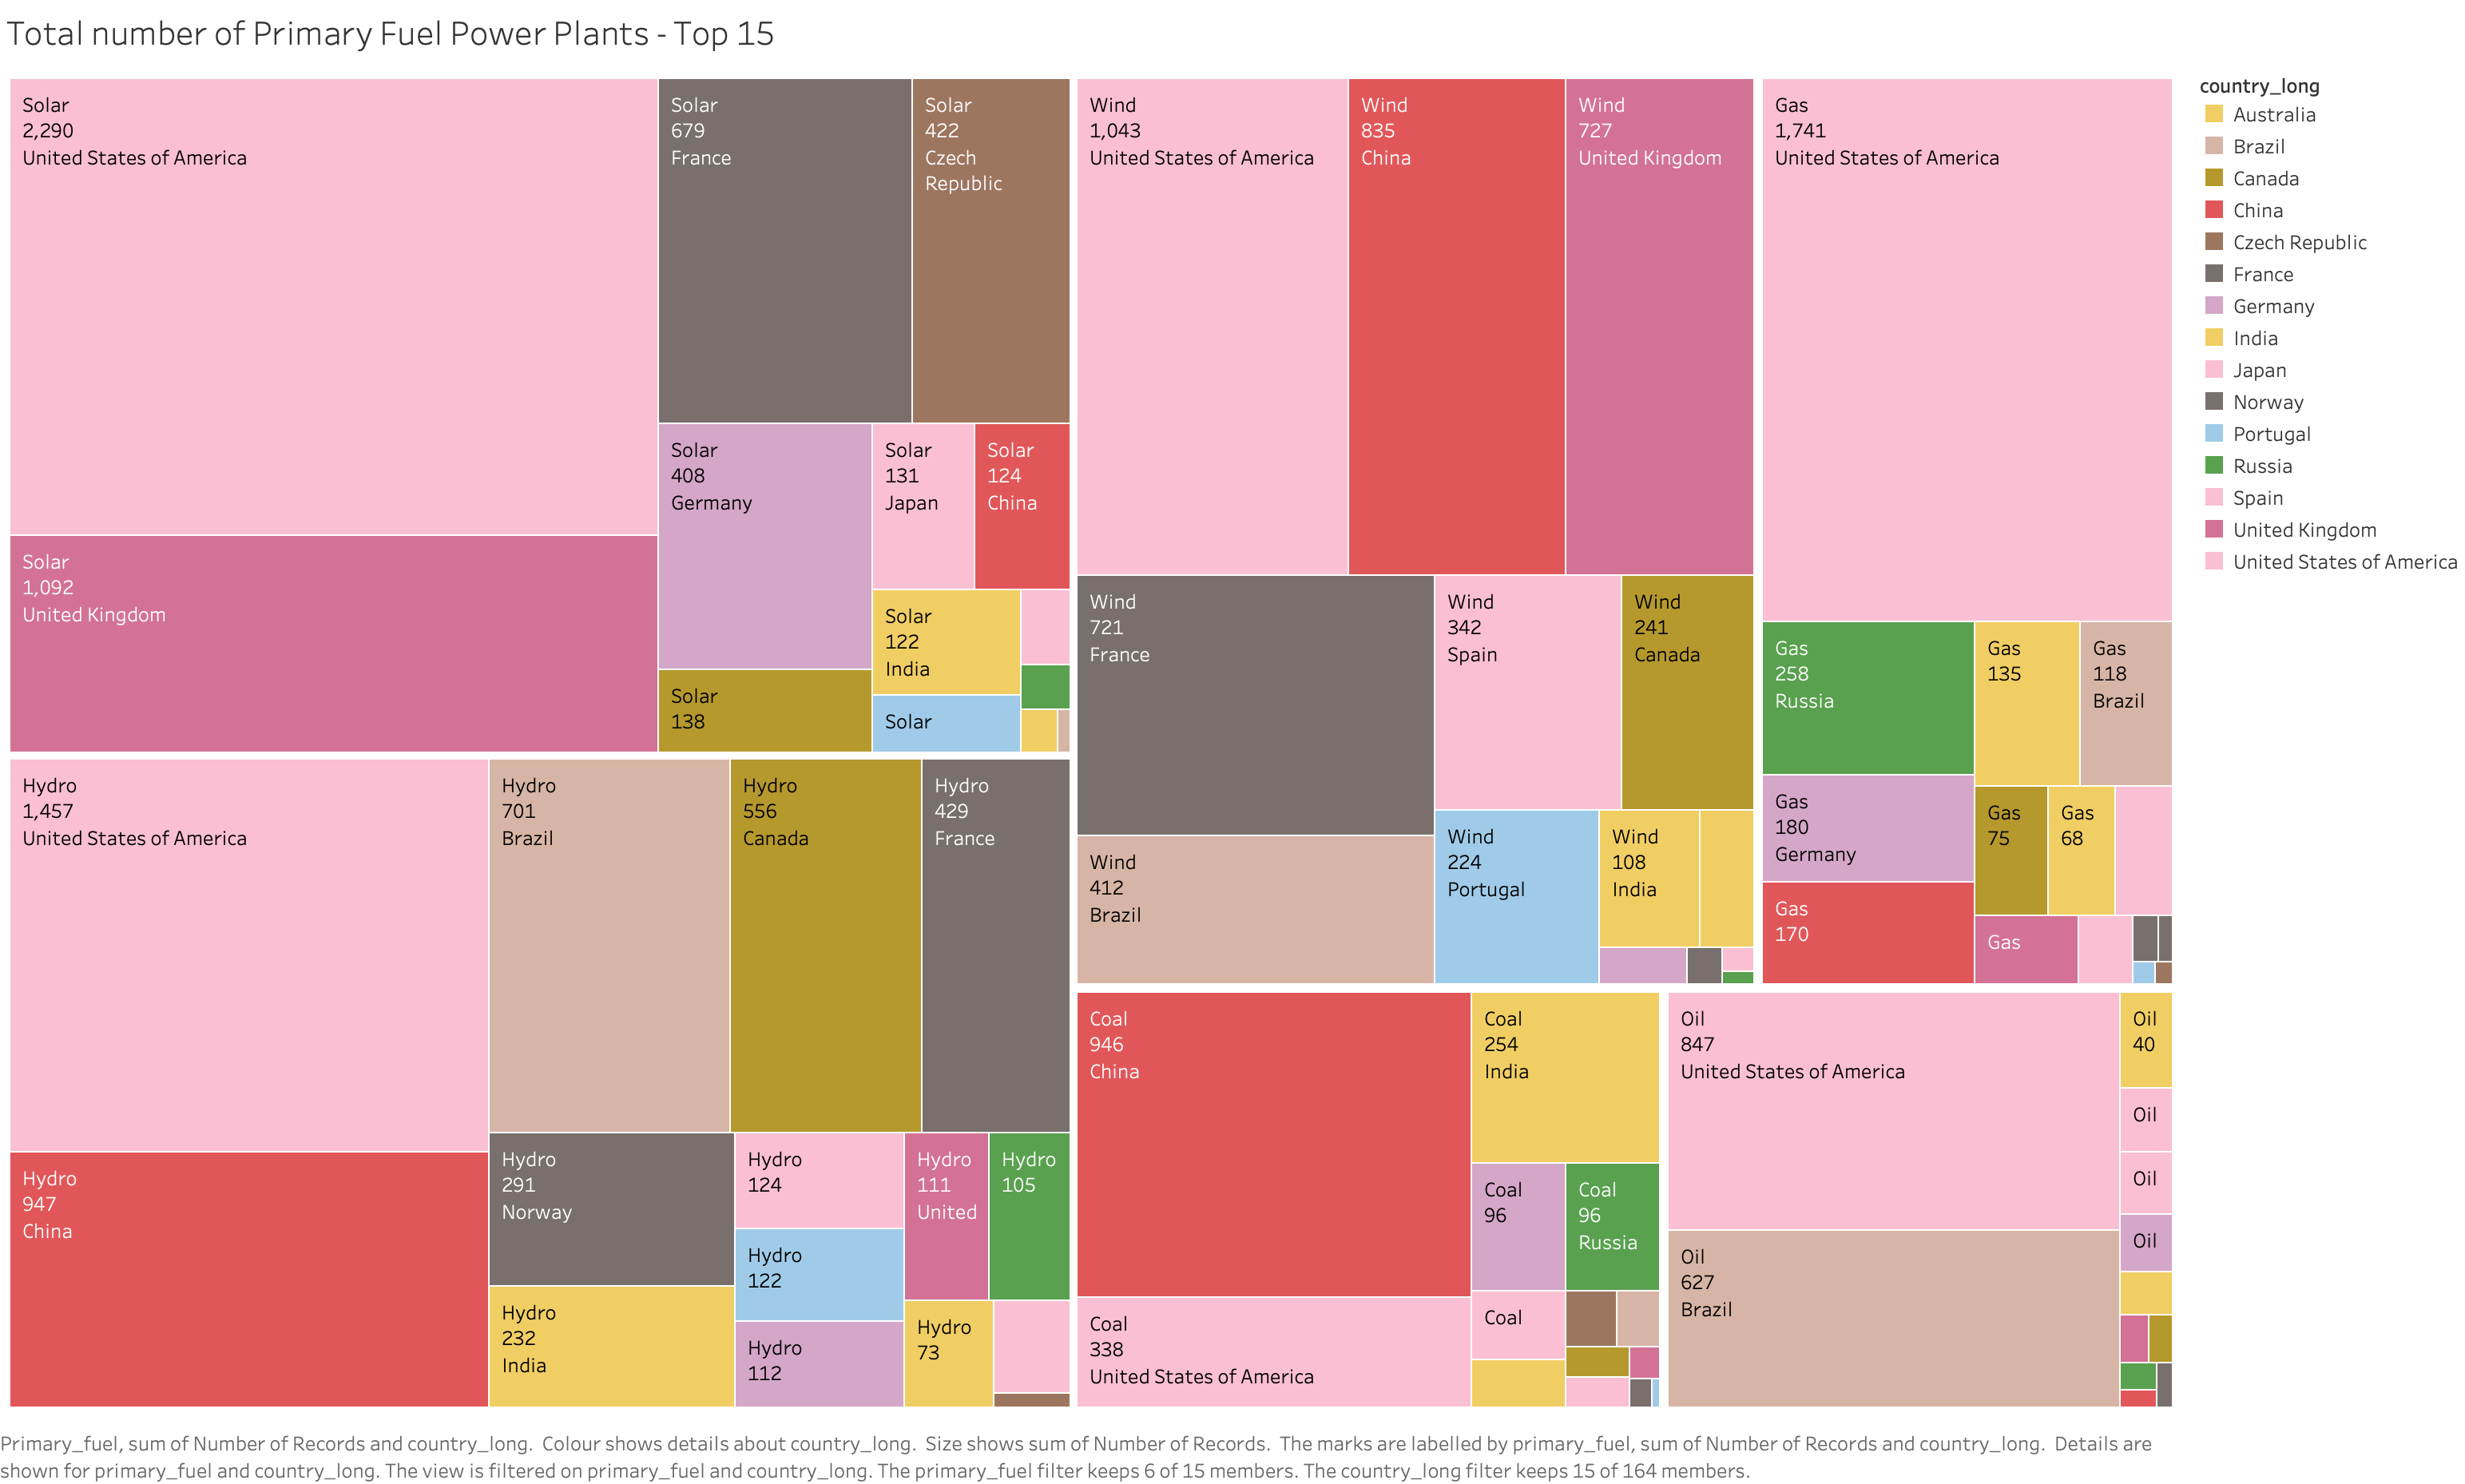
\includegraphics[width=15cm]{Numberofprifueltop15}

\begin{itemize}
\tightlist
\item
  \textbf{Name of Tool}: Tableau
\item
  \textbf{Country}: Australia, Brazil, Canada, China, Czech Republic, France, Germany, India, Japan, Norway, Portugal, Russia, Spain, United Kingdom, USA.
\item
  \textbf{Year}: 1896 - 2018.
\item
  \textbf{Data Preparation}: Top 6 values of the primary fuel was used as well as top 15 filter used for the counteries based on the sum of records.
\item
  \textbf{Color}: Colour has been assissiate to the different counteries.
\item
  \textbf{Hierarchy}: Each hierarchy is linked to the sum of the power plants based on their primary fuel. For example: Solar. 
\item
  What leaf node size is mapped to? This is mapped to the amount of records each country has to the hierarchy primary fuel type.
\item
  How are the leaf nodes laid out or positioned? The leaf nodes are laid out on top of the main hierarchy, each in the shape of a square, with the size of th esquare referencing the size of the record. For example, the bigger the square/rectangle the bigger that record is.
\item
  What are internal nodes mapped to?
\item
  What is internal node size mapped to?
\item
  Which treemap node layout algorithm is used?
  Tableau built in algorithm.
\end{itemize}

\clearpage
\hypertarget{part-3}{%
\section{Part 3}\label{part-3}}

\begin{figure}
\centering
%\includegraphics{screenshotpath}
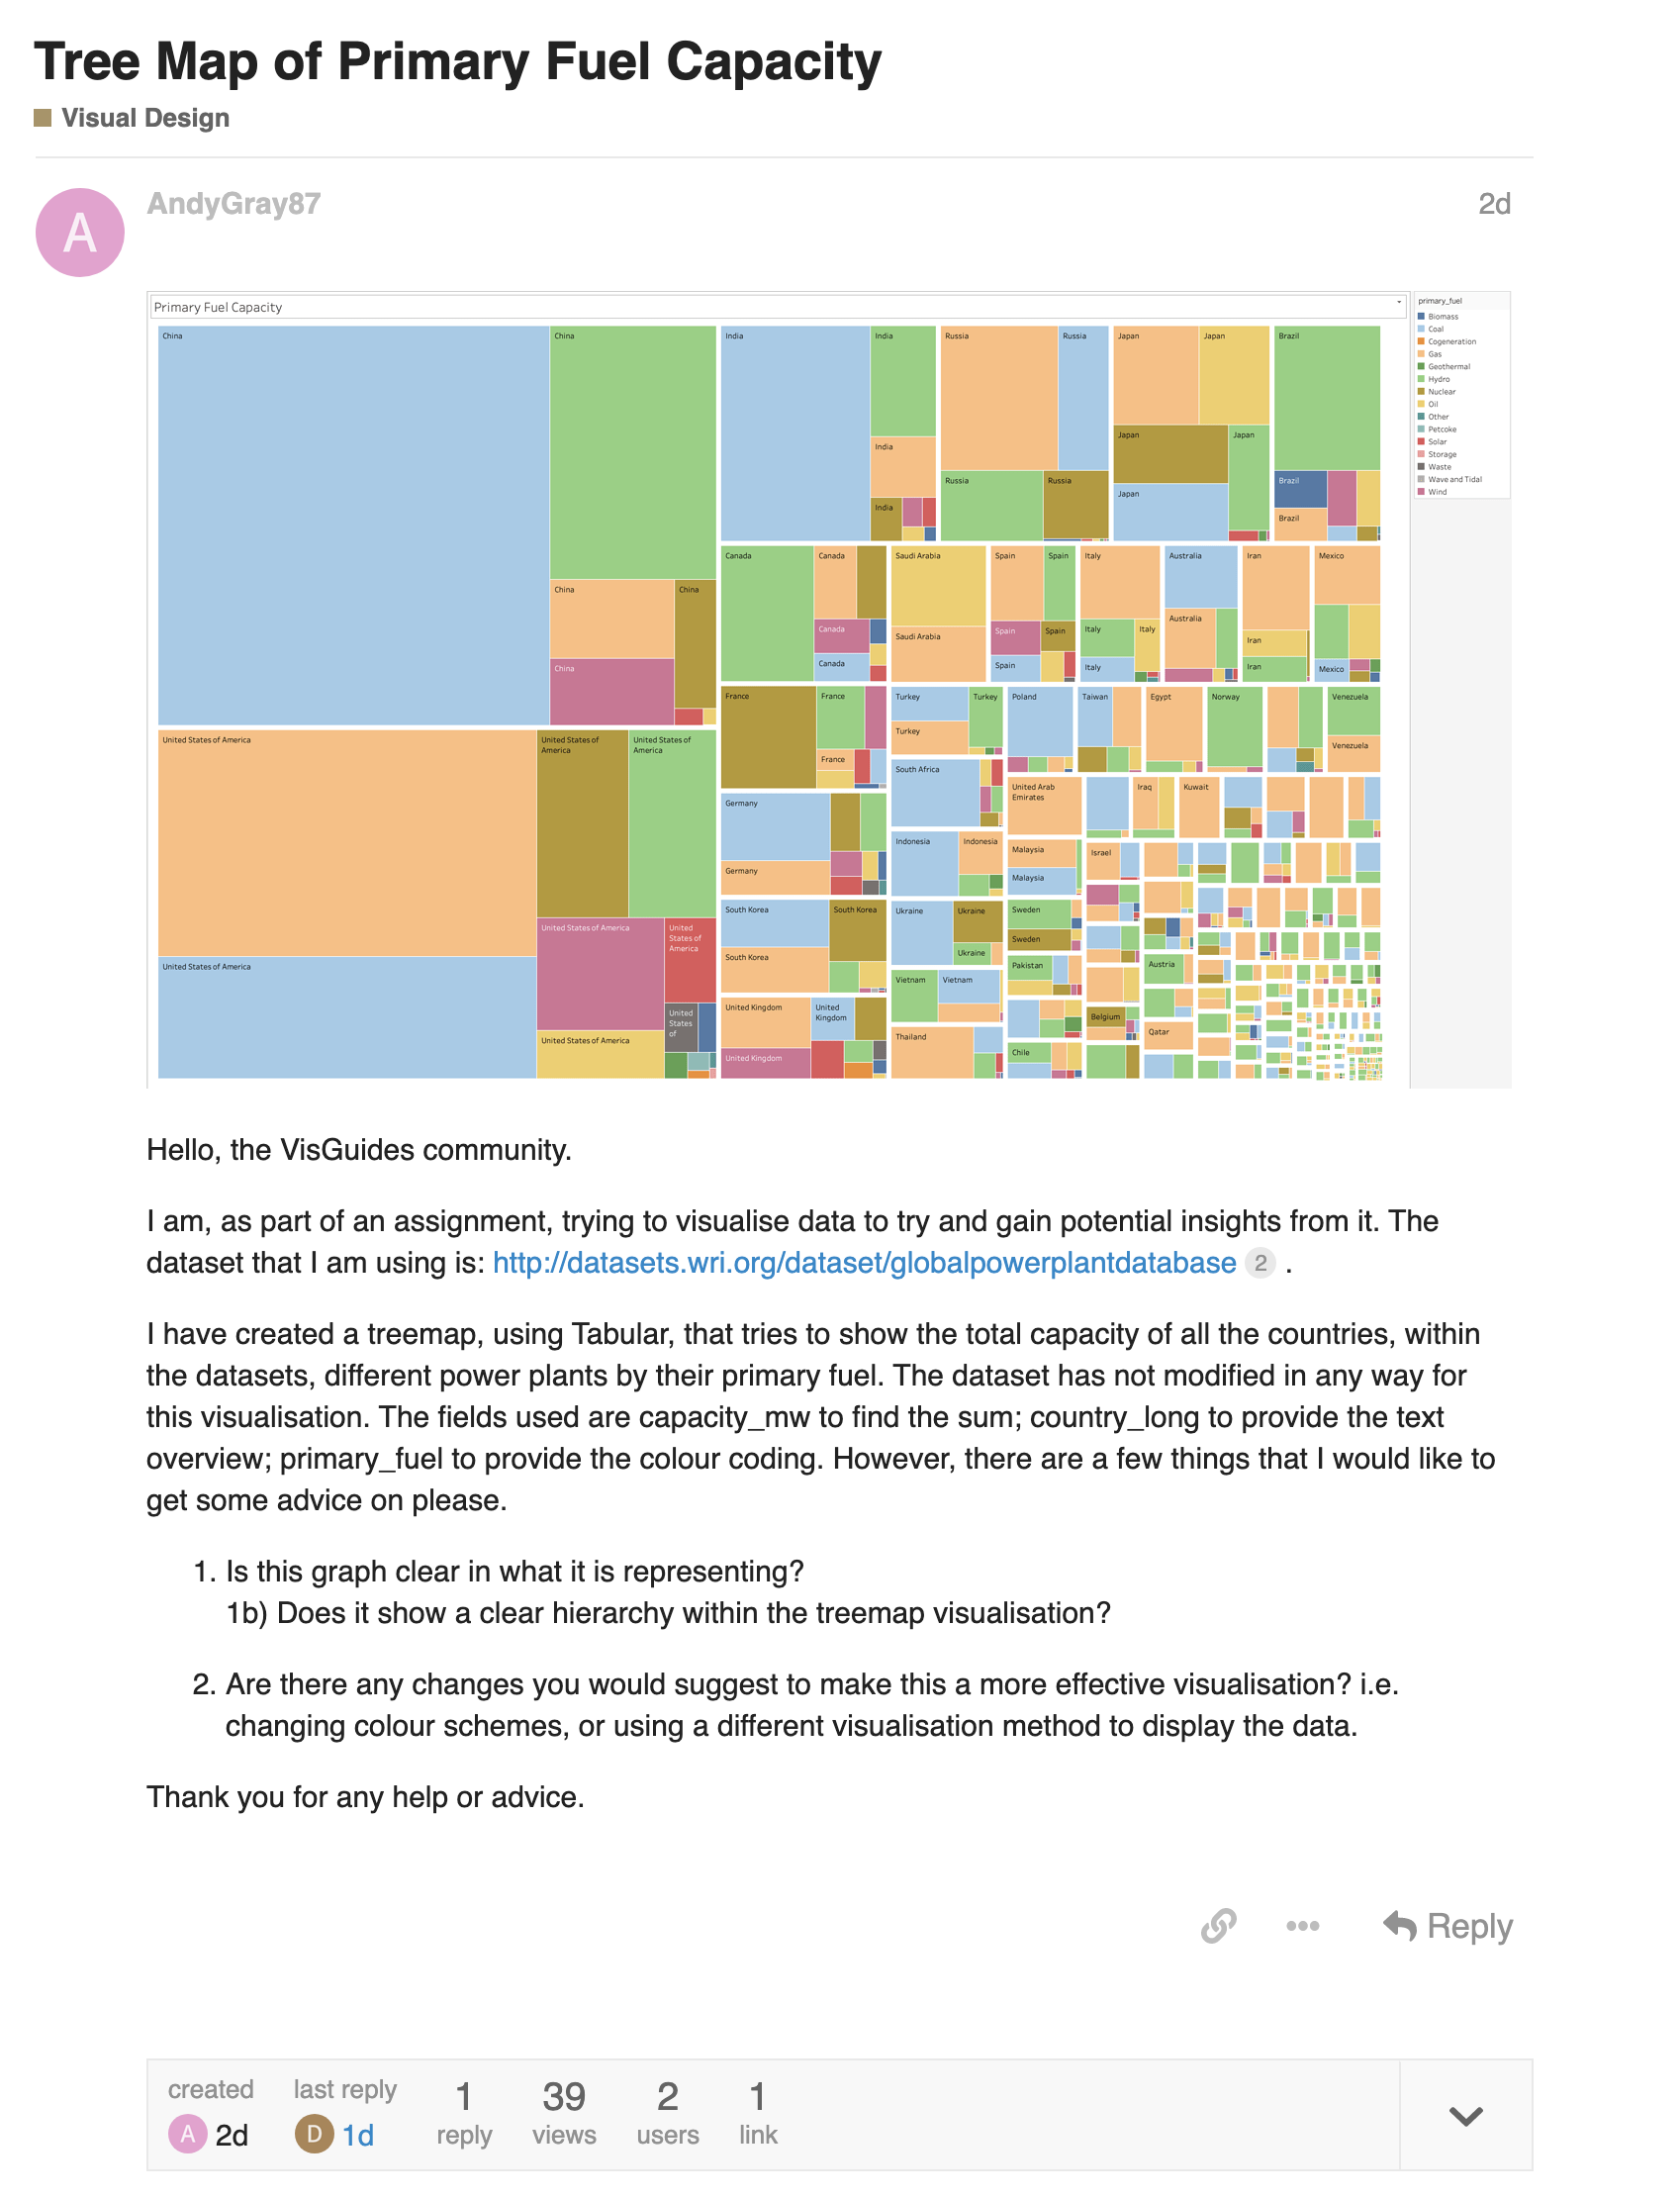
\includegraphics[width=15cm]{Question}
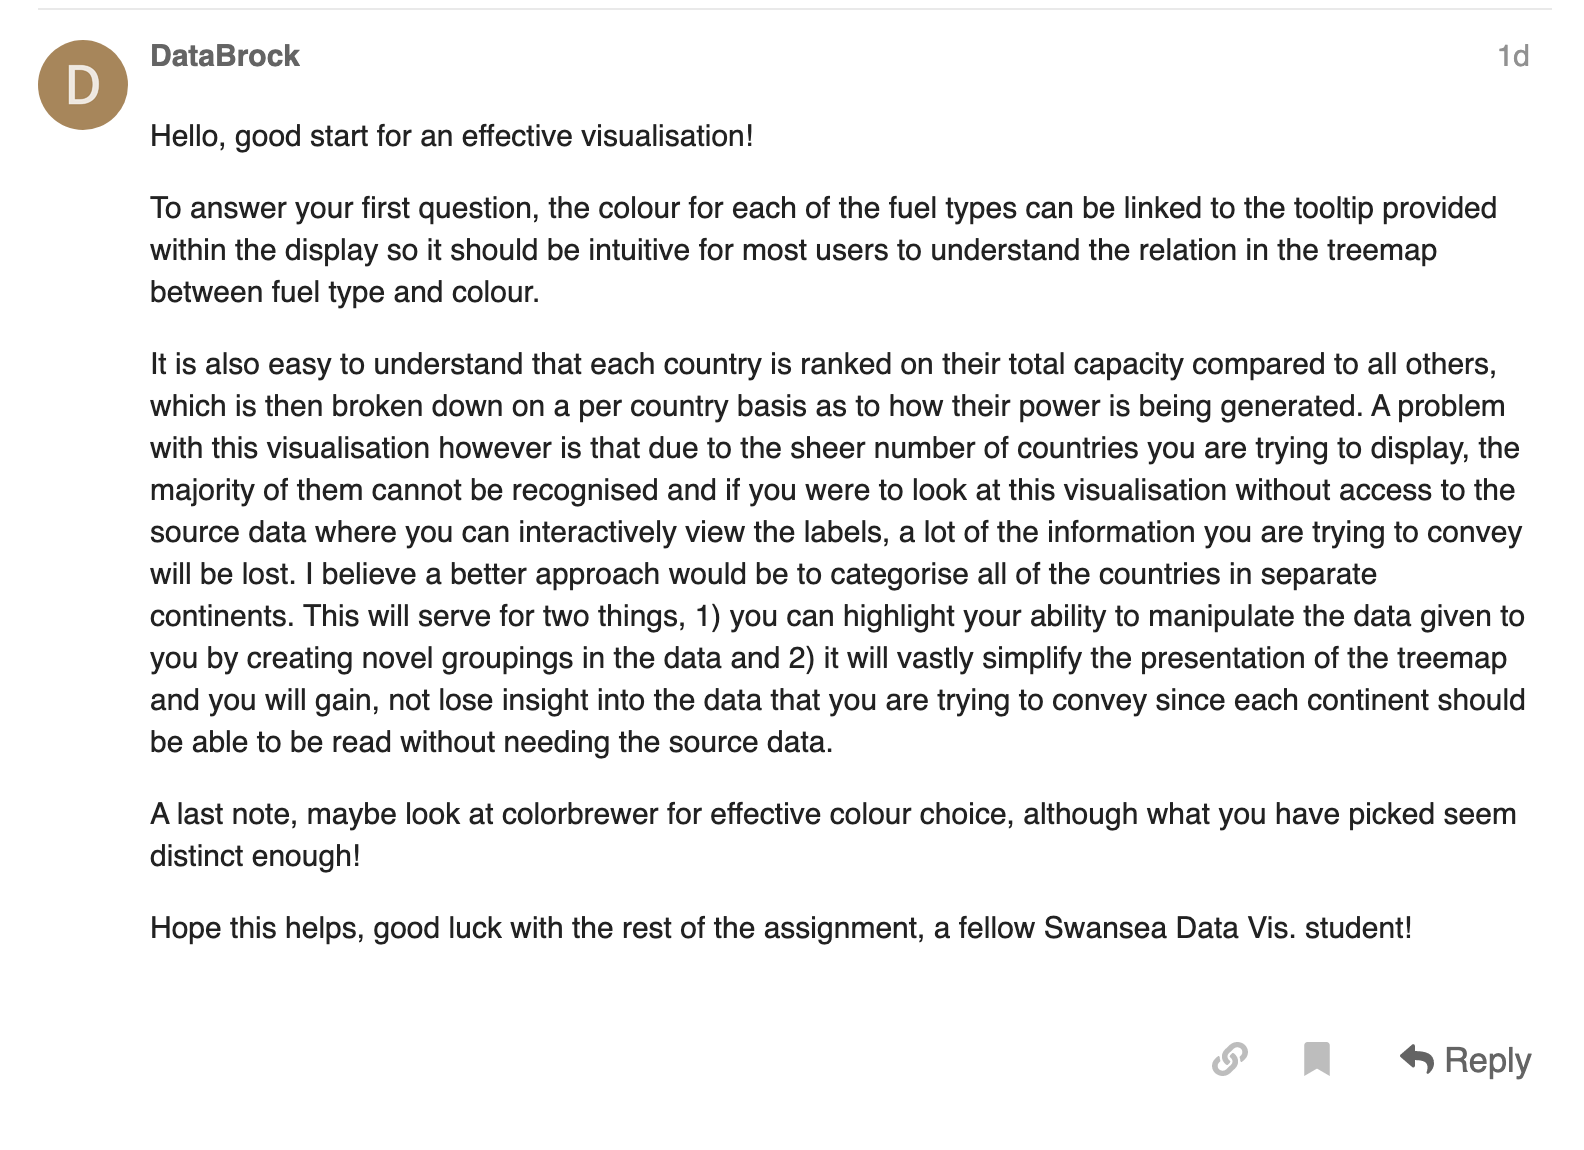
\includegraphics[width=15cm]{answer}
\caption{VisGuides screenshot}
\end{figure}


\end{document}
